\documentclass[border=8pt]{standalone}
\usepackage[T1]{fontenc}\usepackage{helvet}\renewcommand{\familydefault}{\sfdefault}
\usepackage{tikz}\usetikzlibrary{arrows.meta, positioning, calc, backgrounds}
\definecolor{ink}{HTML}{1a1916}
\definecolor{inktwo}{HTML}{3a3a35}
\definecolor{inkthree}{HTML}{6a6862}
\definecolor{rule}{HTML}{b8b09a}
\definecolor{amber}{HTML}{a8730a}
\definecolor{red}{HTML}{c8261a}
\definecolor{paper}{HTML}{f0eee5}
\definecolor{slab}{HTML}{d8d4c6}
\tikzset{
  >={Stealth[length=2.2mm]},
  wire/.style={line width=0.8pt, ink},
  modwire/.style={line width=0.6pt, dashed, ink},
  tastewire/.style={line width=0.6pt, dashed, amber},
  gatewire/.style={line width=0.6pt, dotted, ink},
  block/.style={rectangle, draw=ink, line width=0.9pt, fill=slab, minimum width=3.0cm, minimum height=1.9cm, inner sep=0pt},
  perf/.style={rectangle, draw=ink, line width=0.7pt, minimum width=3.0cm, minimum height=0.7cm, inner sep=2pt, font=\footnotesize, text=ink},
  title/.style={font=\scriptsize\bfseries, text=ink, anchor=north, inner sep=2pt},
  jack/.style={circle, draw=ink, fill=paper, line width=0.5pt, minimum size=3.2pt, inner sep=0pt},
  plabel/.style={font=\tiny, text=inktwo, anchor=west, inner sep=1pt},
  olabel/.style={font=\tiny, text=inktwo, anchor=east, inner sep=1pt},
  settings/.style={font=\scriptsize, text=ink, align=left, anchor=north west, inner sep=1pt, text width=2.9cm},
}
\begin{document}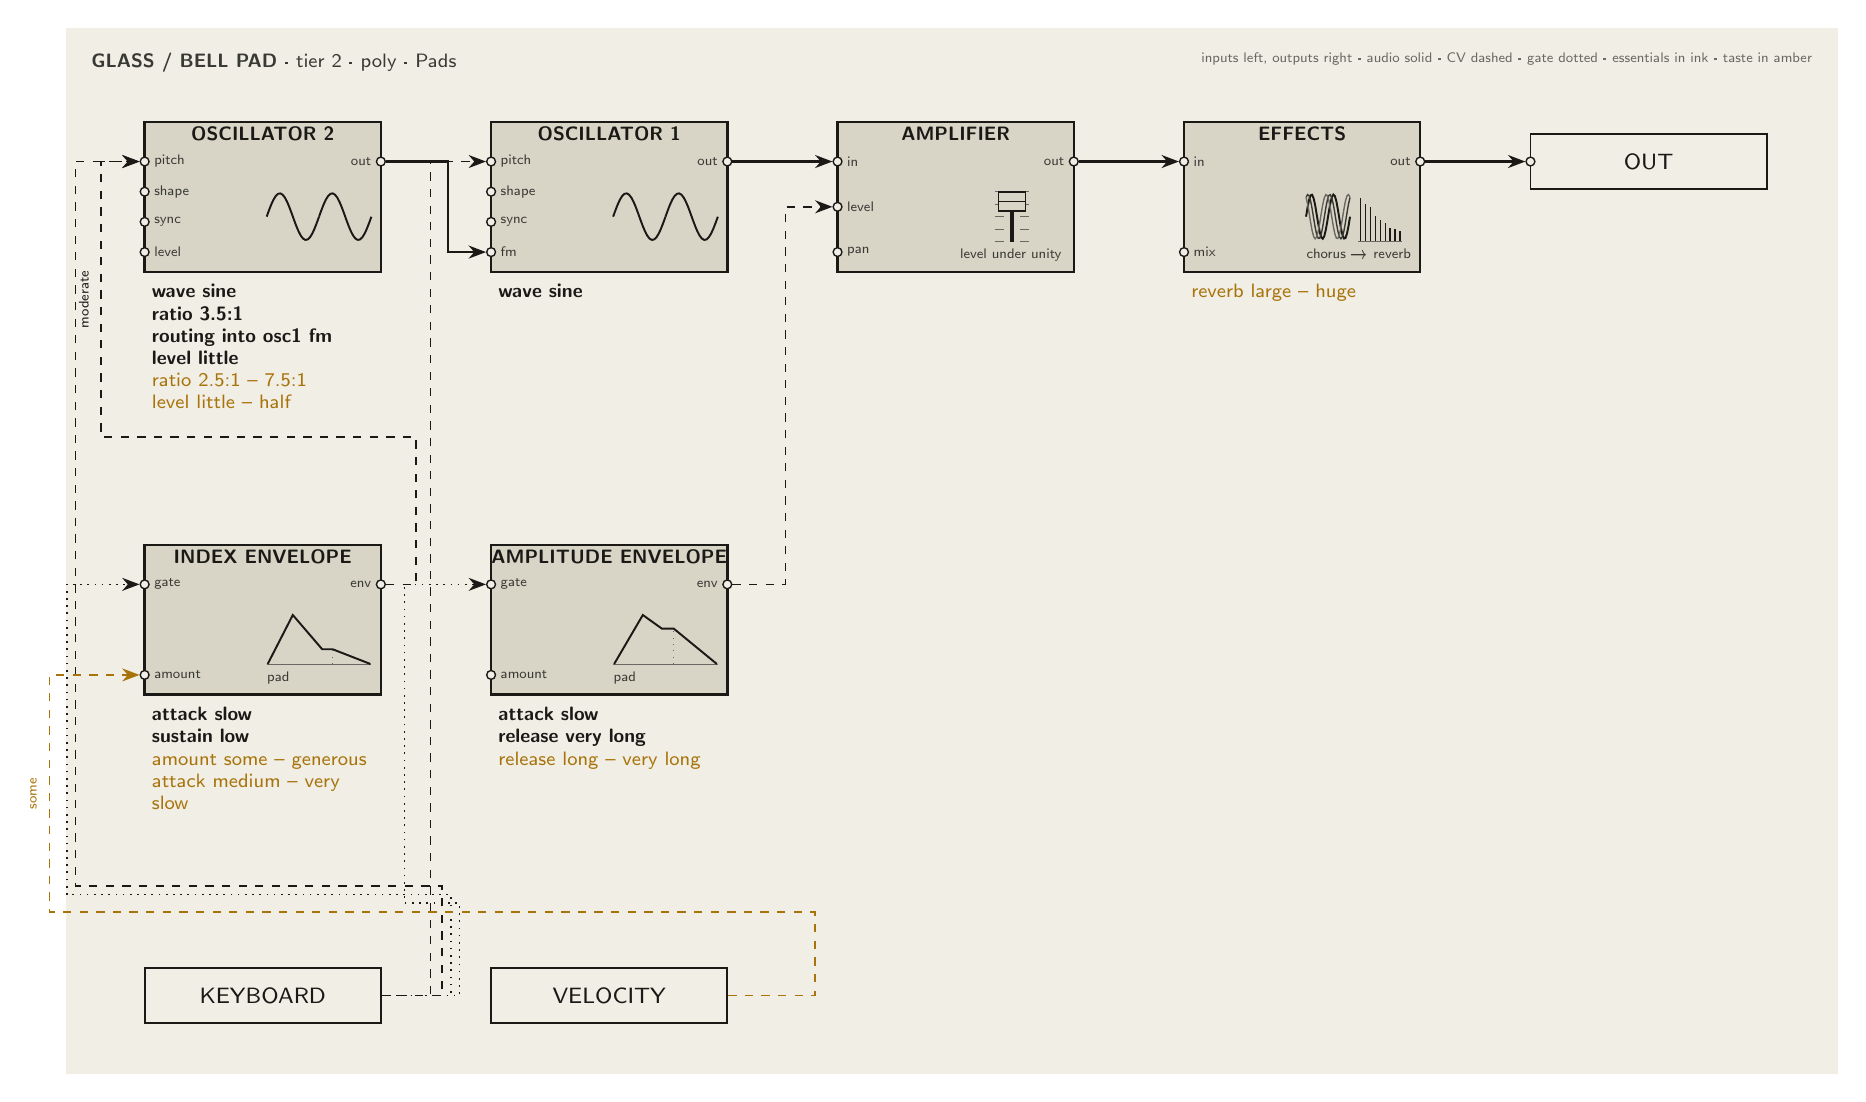
\begin{tikzpicture}
\begin{scope}[on background layer]\fill[paper] (-2.5,-11.139999999999999) rectangle (20.0,2.15);\end{scope}
\node[block, minimum height=1.9cm] (osc1) at (4.4,0.0) {};
\node[title] at (osc1.north) {OSCILLATOR 1};
\node[jack] (osc1-pitch) at (2.9000000000000004,0.44999999999999996) {};
\node[plabel] at (2.9800000000000004,0.44999999999999996) {pitch};
\node[jack] (osc1-shape) at (2.9000000000000004,0.06666666666666665) {};
\node[plabel] at (2.9800000000000004,0.06666666666666665) {shape};
\node[jack] (osc1-sync) at (2.9000000000000004,-0.31666666666666665) {};
\node[plabel] at (2.9800000000000004,-0.31666666666666665) {sync};
\node[jack] (osc1-fm) at (2.9000000000000004,-0.7) {};
\node[plabel] at (2.9800000000000004,-0.7) {fm};
\node[jack] (osc1-out) at (5.9,0.44999999999999996) {};
\node[olabel] at (5.82,0.44999999999999996) {out};
\begin{scope}
\draw[ink, line width=0.7pt] plot[domain=0.000:0.500, samples=24, variable=\u] ({4.450+\u*1.330},{-0.620+(0.740)*(0.5+0.4*sin(360*(\u*2))+0.0)});
\draw[ink, line width=0.7pt] plot[domain=0.500:1.000, samples=24, variable=\u] ({4.450+\u*1.330},{-0.620+(0.740)*(0.5+0.4*sin(360*(\u*2))+0.0)});
\end{scope}
\node[settings] at (2.95,-1.0699999999999998) {\textbf{wave sine}};
\node[block, minimum height=1.9cm] (osc2) at (0.0,0.0) {};
\node[title] at (osc2.north) {OSCILLATOR 2};
\node[jack] (osc2-pitch) at (-1.5,0.44999999999999996) {};
\node[plabel] at (-1.42,0.44999999999999996) {pitch};
\node[jack] (osc2-shape) at (-1.5,0.06666666666666665) {};
\node[plabel] at (-1.42,0.06666666666666665) {shape};
\node[jack] (osc2-sync) at (-1.5,-0.31666666666666665) {};
\node[plabel] at (-1.42,-0.31666666666666665) {sync};
\node[jack] (osc2-level) at (-1.5,-0.7) {};
\node[plabel] at (-1.42,-0.7) {level};
\node[jack] (osc2-out) at (1.5,0.44999999999999996) {};
\node[olabel] at (1.42,0.44999999999999996) {out};
\begin{scope}
\draw[ink, line width=0.7pt] plot[domain=0.000:0.500, samples=24, variable=\u] ({0.050+\u*1.330},{-0.620+(0.740)*(0.5+0.4*sin(360*(\u*2))+0.0)});
\draw[ink, line width=0.7pt] plot[domain=0.500:1.000, samples=24, variable=\u] ({0.050+\u*1.330},{-0.620+(0.740)*(0.5+0.4*sin(360*(\u*2))+0.0)});
\end{scope}
\node[settings] at (-1.45,-1.0699999999999998) {\textbf{wave sine} \\ \textbf{ratio 3.5:1} \\ \textbf{routing into osc1 fm} \\ \textbf{level little} \\ \textcolor{amber}{ratio 2.5:1 -- 7.5:1} \\ \textcolor{amber}{level little -- half}};
\node[block, minimum height=1.9cm] (amp) at (8.8,0.0) {};
\node[title] at (amp.north) {AMPLIFIER};
\node[jack] (amp-in) at (7.300000000000001,0.44999999999999996) {};
\node[plabel] at (7.380000000000001,0.44999999999999996) {in};
\node[jack] (amp-level) at (7.300000000000001,-0.125) {};
\node[plabel] at (7.380000000000001,-0.125) {level};
\node[jack] (amp-pan) at (7.300000000000001,-0.7) {};
\node[plabel] at (7.380000000000001,-0.7) {pan};
\node[jack] (amp-out) at (10.3,0.44999999999999996) {};
\node[olabel] at (10.22,0.44999999999999996) {out};
\begin{scope}
\draw[ink, line width=1.2pt] (9.515,-0.570) -- (9.515,0.070);
\draw[inkthree, line width=0.3pt] (9.295,-0.570) -- (9.415,-0.570) (9.615,-0.570) -- (9.735,-0.570);
\draw[inkthree, line width=0.3pt] (9.295,-0.410) -- (9.415,-0.410) (9.615,-0.410) -- (9.735,-0.410);
\draw[inkthree, line width=0.3pt] (9.295,-0.250) -- (9.415,-0.250) (9.615,-0.250) -- (9.735,-0.250);
\draw[inkthree, line width=0.3pt] (9.295,-0.090) -- (9.415,-0.090) (9.615,-0.090) -- (9.735,-0.090);
\draw[inkthree, line width=0.3pt] (9.295,0.070) -- (9.415,0.070) (9.615,0.070) -- (9.735,0.070);
\fill[slab, draw=ink, line width=0.6pt] (9.345,-0.178) rectangle (9.685,0.062);
\draw[ink, line width=0.5pt] (9.345,-0.058) -- (9.685,-0.058);
\node[font=\tiny, text=inktwo, anchor=north west, inner sep=0pt] at (8.850,-0.650) {level under unity};
\end{scope}
\node[block, minimum height=1.9cm] (fx) at (13.200000000000001,0.0) {};
\node[title] at (fx.north) {EFFECTS};
\node[jack] (fx-in) at (11.700000000000001,0.44999999999999996) {};
\node[plabel] at (11.780000000000001,0.44999999999999996) {in};
\node[jack] (fx-mix) at (11.700000000000001,-0.7) {};
\node[plabel] at (11.780000000000001,-0.7) {mix};
\node[jack] (fx-out) at (14.700000000000001,0.44999999999999996) {};
\node[olabel] at (14.620000000000001,0.44999999999999996) {out};
\begin{scope}
\draw[ink, line width=0.7pt] plot[domain=0.000:0.420, samples=30, variable=\u] ({13.250+\u*1.330},{-0.620+(0.740)*(0.5+0.38*sin(360*((\u-0.000)/0.420)*2+0))});
\draw[inktwo, line width=0.5pt] plot[domain=0.000:0.420, samples=30, variable=\u] ({13.250+\u*1.330},{-0.620+(0.740)*(0.5+0.38*sin(360*((\u-0.000)/0.420)*2+60))});
\draw[inkthree, line width=0.5pt] plot[domain=0.000:0.420, samples=30, variable=\u] ({13.250+\u*1.330},{-0.620+(0.740)*(0.5+0.38*sin(360*((\u-0.000)/0.420)*2+120))});
\draw[inkthree, line width=0.3pt] (13.915,-0.561) -- (14.474,-0.561);
\draw[ink, line width=0.6pt] (13.943,-0.561) -- (13.943,-0.018);
\draw[ink, line width=0.6pt] (14.006,-0.561) -- (14.006,-0.095);
\draw[ink, line width=0.6pt] (14.069,-0.561) -- (14.069,-0.133);
\draw[ink, line width=0.6pt] (14.131,-0.561) -- (14.131,-0.246);
\draw[ink, line width=0.6pt] (14.194,-0.561) -- (14.194,-0.296);
\draw[ink, line width=0.6pt] (14.257,-0.561) -- (14.257,-0.335);
\draw[ink, line width=0.6pt] (14.320,-0.561) -- (14.320,-0.394);
\draw[ink, line width=0.6pt] (14.383,-0.561) -- (14.383,-0.408);
\draw[ink, line width=0.6pt] (14.446,-0.561) -- (14.446,-0.429);
\node[font=\tiny, text=inktwo, anchor=north west, inner sep=0pt] at (13.250,-0.650) {chorus → reverb};
\end{scope}
\node[settings] at (11.750000000000002,-1.0699999999999998) {\textcolor{amber}{reverb large -- huge}};
\node[block, minimum height=1.9cm] (menv) at (0.0,-5.37) {};
\node[title] at (menv.north) {INDEX ENVELOPE};
\node[jack] (menv-gate) at (-1.5,-4.92) {};
\node[plabel] at (-1.42,-4.92) {gate};
\node[jack] (menv-amount) at (-1.5,-6.07) {};
\node[plabel] at (-1.42,-6.07) {amount};
\node[jack] (menv-out) at (1.5,-4.92) {};
\node[olabel] at (1.42,-4.92) {env};
\begin{scope}
\draw[inkthree, line width=0.3pt] (0.050,-5.931) -- (1.380,-5.931);
\draw[ink, line width=0.7pt] (0.063,-5.931) -- (0.382,-5.309) -- (0.755,-5.744) -- (0.888,-5.744) -- (1.367,-5.931);
\draw[inkthree, line width=0.3pt, dotted] (0.888,-5.931) -- (0.888,-5.744);
\node[font=\tiny, text=inktwo, anchor=north west, inner sep=0pt] at (0.050,-6.020) {pad};
\end{scope}
\node[settings] at (-1.45,-6.44) {\textbf{attack slow} \\ \textbf{sustain low} \\ \textcolor{amber}{amount some -- generous} \\ \textcolor{amber}{attack medium -- very slow}};
\node[block, minimum height=1.9cm] (aenv) at (4.4,-5.37) {};
\node[title] at (aenv.north) {AMPLITUDE ENVELOPE};
\node[jack] (aenv-gate) at (2.9000000000000004,-4.92) {};
\node[plabel] at (2.9800000000000004,-4.92) {gate};
\node[jack] (aenv-amount) at (2.9000000000000004,-6.07) {};
\node[plabel] at (2.9800000000000004,-6.07) {amount};
\node[jack] (aenv-out) at (5.9,-4.92) {};
\node[olabel] at (5.82,-4.92) {env};
\begin{scope}
\draw[inkthree, line width=0.3pt] (4.450,-5.931) -- (5.780,-5.931);
\draw[ink, line width=0.7pt] (4.463,-5.931) -- (4.827,-5.309) -- (5.070,-5.483) -- (5.221,-5.483) -- (5.767,-5.931);
\draw[inkthree, line width=0.3pt, dotted] (5.221,-5.931) -- (5.221,-5.483);
\node[font=\tiny, text=inktwo, anchor=north west, inner sep=0pt] at (4.450,-6.020) {pad};
\end{scope}
\node[settings] at (2.95,-6.44) {\textbf{attack slow} \\ \textbf{release very long} \\ \textcolor{amber}{release long -- very long}};
\node[perf] (key) at (0.0,-10.139999999999999) {KEYBOARD};
\node[perf] (vel) at (4.4,-10.139999999999999) {VELOCITY};
\node[perf, fill=paper] (out) at (17.6,0.44999999999999996) {OUT}; \node[jack] (out-in) at (16.1,0.44999999999999996) {};
\draw[wire,->] (osc2-out) -- (2.3500000000000005,0.44999999999999996) -- (2.3500000000000005,-0.7) -- (osc1-fm);
\draw[wire,->] (osc1-out) -- (amp-in);
\draw[wire,->] (amp-out) -- (fx-in);
\draw[wire,->] (fx-out) -- (out-in);
\draw[modwire,->] (menv-out) -- (1.95,-4.92) -- (1.95,-3.05) -- (-2.05,-3.05) -- (-2.05,0.44999999999999996) -- (osc2-pitch);
\node[font=\tiny, text=ink, anchor=south, inner sep=1pt, rotate=90] at (-2.17,-1.2999999999999998) {moderate};
\draw[modwire,->] (aenv-out) -- (6.640000000000001,-4.92) -- (6.640000000000001,-0.125) -- (amp-level);
\draw[modwire,->] (key.east) -- (2.1300000000000003,-10.139999999999999) -- (2.1300000000000003,0.44999999999999996) -- (osc1-pitch);
\draw[modwire,->] (key.east) -- (2.28,-10.139999999999999) -- (2.28,-8.75) -- (-2.38,-8.75) -- (-2.38,0.44999999999999996) -- (osc2-pitch);
\draw[gatewire,->] (key.east) -- (2.39,-10.139999999999999) -- (2.39,-8.86) -- (-2.4899999999999998,-8.86) -- (-2.4899999999999998,-4.92) -- (menv-gate);
\draw[gatewire,->] (key.east) -- (2.5,-10.139999999999999) -- (2.5,-8.97) -- (1.8000000000000005,-8.97) -- (1.8000000000000005,-4.92) -- (aenv-gate);
\draw[tastewire,->] (vel.east) -- (7.010000000000001,-10.139999999999999) -- (7.010000000000001,-9.08) -- (-2.71,-9.08) -- (-2.71,-6.07) -- (menv-amount);
\node[font=\tiny, text=amber, anchor=south, inner sep=1pt, rotate=90] at (-2.83,-7.575) {some};
\node[anchor=north west, font=\scriptsize, text=inktwo] at (-2.3,1.95) {\textbf{GLASS / BELL PAD} · tier 2 · poly · Pads};
\node[anchor=north east, font=\tiny, text=inkthree] at (19.8,1.95) {inputs left, outputs right · audio solid · CV dashed · gate dotted · essentials in ink · taste in amber};
\end{tikzpicture}\end{document}
